\section{Experiments}
Our experiments are designed to address the following questions:
\begin{enumerate}
    \renewcommand{\labelenumi}{\roman{enumi})}
    \item Does \method produce more natural behaviors than unregularized counterparts?
    \item Does \method achieve gains in performance comparing with other exploration strategies? %via efficient exploration
    \item Does \method enable effective transfer from simulation to real-world hardware?
\end{enumerate}
\paragraph{Environment.} All experiments are conducted in IsaacLab simulation environment~\citep{mittal2025isaaclab}. We use the Unitree Go2 quadruped robot with $12$ degrees of freedom. The action space is defined as $\mathcal{A} \subseteq [-1, +1]^{12}$. The simulation runs at $200$\,Hz, while the PD controller operates at $50$\,Hz. Details about state space and domain randomization can be found in \Cref{appendix:observation-space}.

\paragraph{Task Metrics.}
We evaluate \method on two different sets of downstream tasks: velocity-tracking tasks and base orientation tasks. Both the velocity-tracking and base-orientation settings consists of $17$ downstream tasks. Performance is measured by the average episode return achieved on each task, with the episode length equals 250 steps and a maximum achievable reward of $250$. Detailed downstream task reward are in appendix \Cref{appendix:reward-function}. We additionally report the foot sliding to assess locomotion quality (details in \Cref{appendix:regularization_reward}).

\paragraph{Baselines.} We compare \method with several baselines and ablations. FB \citep{touati2021learning} performs undirected exploration by uniformly sampling random reward embeddings from the hypersphere. FB-Critic uses the same uniform exploration strategy as FB but includes our proposed behavior regularizer (see \Cref{sec:limitations}). This isolates the performance gains provided by our exploration strategy from the gains provided by the regularizer. \method ($\beta$=2, our method) includes a behavior regularizer and directs exploration sampling 80\% of its embeddings with our proposed MEBE strategy (\Cref{eq:practical_fb_mebe}) and 20\% using uniform random embeddings. Finally, we include an ablation FB-MEBE ($\beta$=0), which sets the reverse sampling coefficient $\beta$ to zero. This can be seen as an instantiation of FB-CPR \citep{tirinzoni2025zeroshot}, with no data prior. Instead of prioritizing rare behaviors, it performs uniform exploration over the achieved behaviors.  This isolates the performance gains provided by our exploration strategy from the gains provided by the biasing towards goal-reaching behaviors. For other ablations on the $\beta$ parameter and on sampling strategies, see \Cref{appendix:ablation_beta,appendix:ablation_exptrain}, respectively.

In practice, to focus exploration on relevant parts of the state space, we conduct exploration over a lower-dimensional projections of the state rather than directly operating on the full state space. Formally we define a projection mapping $\varphi: S \rightarrow S'$, where $S\subseteq\sR^d, S' \subseteq \sR^{m}, m<d$. For velocity-tracking tasks, exploration is performed in the planar base velocity space $\left[v_x, v_y\right]$. For base-orientation tasks exploration is performed in the space of the gravity vector expressed in the robot base frame $\left[g_x, g_y, g_z\right]$, which characterizes the base orientation. While this restricts the exploration scop to task-relevant settings, \method could be easily extended to operate directly on the full state-space, which we leave for future work.  

% \todo{Add the Vxy filtering in appendix, maybe later use FB-MEBE without filtering so we don't need to introduce filtering}

\subsection{Main Results}
\begin{figure}[H]
    \centering
    \begin{minipage}{\textwidth}
    \centering
    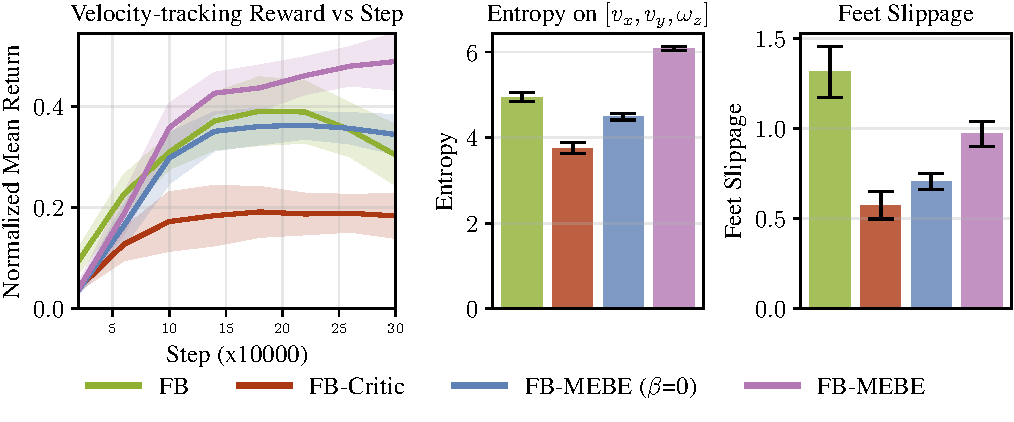
\includegraphics[width=0.8\linewidth]{figure/locomotion_list_mean_fast_td3_exp_and_train.pdf}
    \end{minipage}
% \end{figure}

% \begin{figure}[H]
    \begin{minipage}{\textwidth}
    \centering
    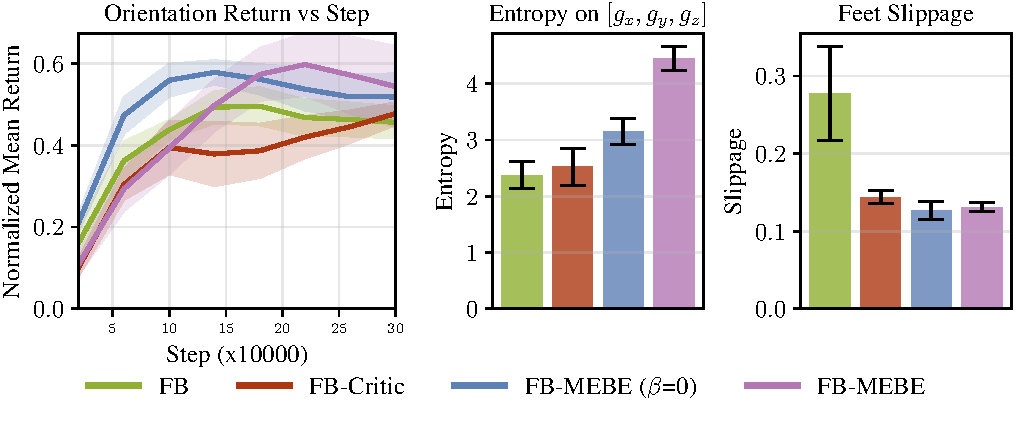
\includegraphics[width=0.8\linewidth]{figure/orientation_list_mean_fast_td3_exp_and_train.pdf}
    \end{minipage}
    \caption{
    Left: Zero-shot performance averaged over 17 downstream velocity tracking tasks (top) and orientation tasks (bottom). We plot normalized return wrt the mean return of Fast-TD3 \citep{seo-2025}. 
    Results are averaged across 5 random seeds, with shaded regions indicating $\pm$ 1-standard deviation. 
    Middle: Policy entropy on $\left[v_x, v_y, w_z \right]$ (top)  and $\left[g_x, g_y, g_z\right]$ (bottom) measured at 300K training steps. (Higher is better). 
    Right: Feet slippage measured at 300K training steps. (Lower is better).}
    \label{fig:FB-MEBE}
\end{figure}

\paragraph{Overall Performance.}
In \Cref{fig:FB-MEBE}, we report results on several downstream tasks. All returns are normalized using the mean return achieved by Fast-TD3 \citep{seo-2025}. Fast-TD3 is a supervised reinforcement learning algorithm trained directly with task-specific rewards, and therefore serves as an approximate upper bound under explicit reward supervision. In contrast, all FB-based methods are trained without access to downstream task rewards and must rely on unsupervised exploration to acquire useful behaviors. %As a result, their performance is naturally lower than that of Fast-TD3.
 \method achieves an average performance that is the highest over all the other baselines for velocity tracking tasks or on par with best performing baseline for orientation tasks. Most notably, it yields the highest entropy among all baselines. This indicates that \method expands behavioral coverage during online training. Importantly, this broader exploration translates into improved downstream task performance rather than unstructured behavior diversification. This can be further seen in \Cref{fig:FB-MEBE-Detailed-Perforance,fig:orientation} where \method outperforms all other baselines in extreme downstream tasks. For orientation tasks, \method shows lower sample efficiency than \method-$\beta=0$, showcasing that unprioritized goal-reaching exploration can be a valid strategy for some downstream tasks. In contrast, FB and FB Critic performs the worst among all algorithms, which we attribute to uninformed exploration (FB) and the additional regularization constraints (FB-critic) that overly restrict exploration, specially in velocity-tracking tasks, leading to limited behavioral coverage and consequently lower average performance.  Regarding gait-related metrics, FB-MEBE substantially reduces the feet slide penalty compared to the original FB, indicating that the regularization critic successfully suppresses unnatural dragging behaviors. Although FB-MEBE exhibits slightly higher feet slippage than FB-Critic, this difference is expected. Since FB-MEBE actively explores higher locomotion velocities, increased horizontal foot velocities naturally lead to higher sliding penalties. Therefore, the observed difference reflects expanded behavioral coverage rather than degraded gait stability. %Overall, FB-MEBE achieves a better balance between exploration capacity and task performance.

%%%%%%%%%%%%%%%%%%%%%%%%%%%%%%%%%%%
\paragraph{Detailed Locomotion Performance.}
\Cref{fig:FB-MEBE-Detailed-Perforance} reports performance across 17 velocity-tracking tasks. 
For moderate velocity commands, all methods obtain reasonable returns. However, for high-velocity tasks, all baselines suffer noticeable performance degradation. This phenomenon is consistent with the replay buffer distribution shown in \Cref{appendix:replay_buffer_data_distribution}, where naive online FB training (FB baseline) progressively concentrates data in low-velocity regions. This distributional shrinkage leads to insufficient coverage of high-speed behaviors and limits zero-shot performance to boundary velocity tasks. By contrast, FB-MEBE expands the replay buffer coverage tencouraging exploration in sparsely visited velocity regions. Consequently, FB-MEBE maintains strong performance even on boundary tasks, demonstrating improved downstream performance.

\begin{figure}[H]
    \centering
    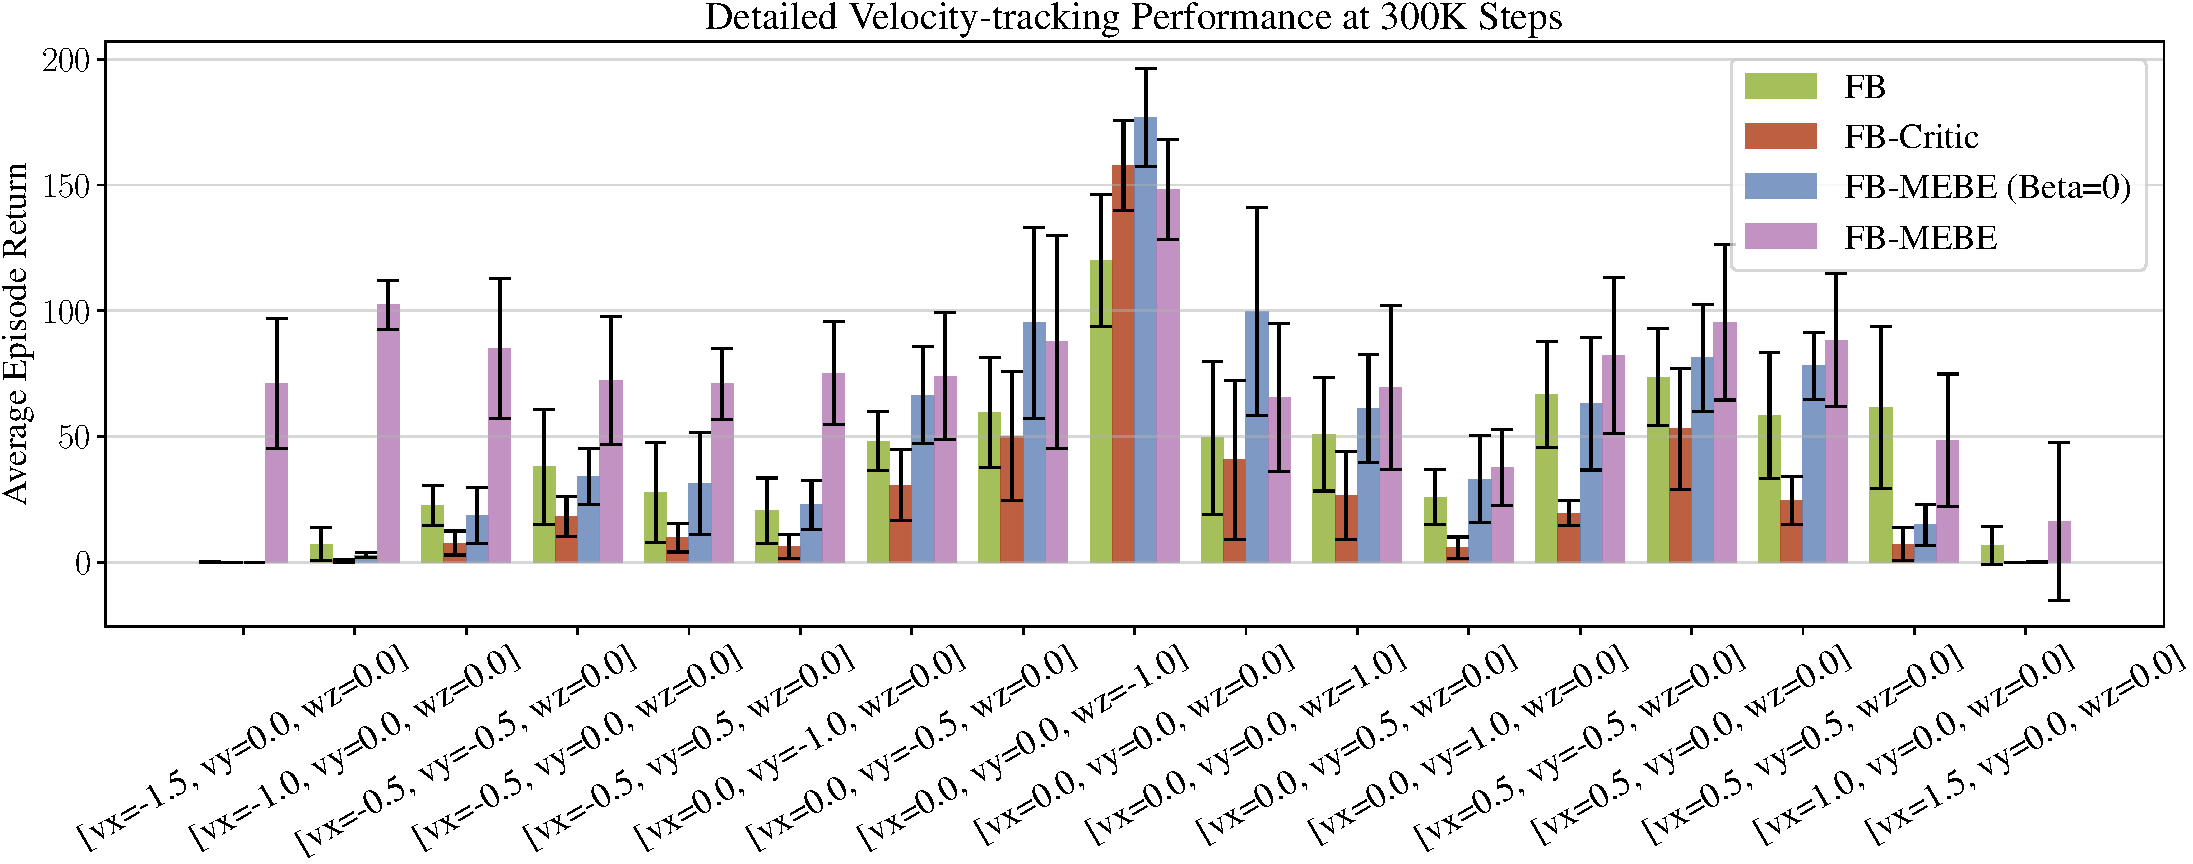
\includegraphics[width=1.0\linewidth]{figure/comparison_detailed_locomotion_task_exp_and_train.pdf}
    \caption{
    Comparison of different methods under detailed locomotion command settings. 
    Each group on the x-axis corresponds to a target velocity command $[v_x, v_y, \omega_z]$. 
    The y-axis reports the mean episode return evaluated under the reward function (in \Cref{appendix:reward-function}) associated with the corresponding target velocity. 
    Results are averaged over 5 random seeds, and error bars denote $\pm$ 1-standard deviation.
    }
    \label{fig:FB-MEBE-Detailed-Perforance}
\end{figure}
\paragraph{Detailed Orientation Performance.}
\Cref{fig:orientation} shows the performance across 12 base orientation tracking settings. 
Notably, \method demonstrates superior performance on challenging large-angle tasks compared to baselines. This indicates enhanced exploration within the orientation behavior space.
However, we observe that FB-MEBE achieves lower returns than baselines on small-angle orientation tasks, including FB-critic (which could be due to the behavior regularization not impeding exploration for orientation tasks). This suggests that \method allocates more model capacity towards extreme behaviors. Balancing this capacity, could be addressed through further finetuning of the exploration ratio.
\begin{figure}[t]
    \centering
    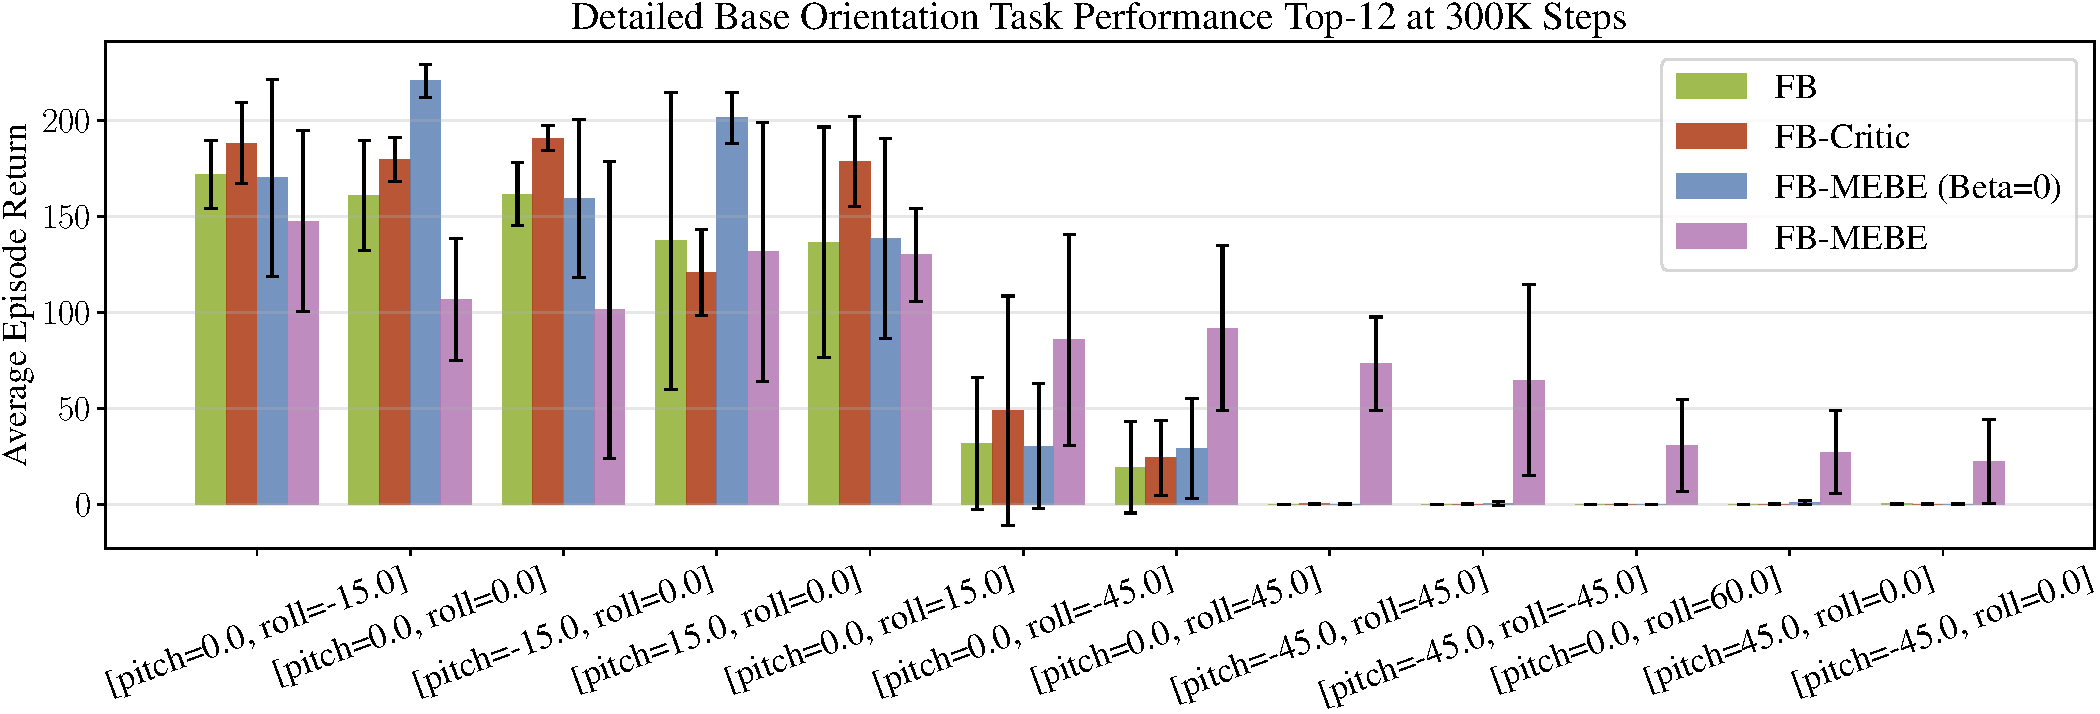
\includegraphics[width=1.0\linewidth]{figure/comparison_detailed_orientation_task_exp_and_train.pdf}
    \caption{
    Comparison of different methods under detailed orientation command settings. Each group on the x-axis corresponds to a target orientation command $[\text{Pitch}, \text{Roll}]$. We removed tasks for which all algorithms get rewards smaller than one from the graph.
    % The y-axis reports the mean episode return evaluated under the reward function (in \Cref{appendix:reward-function}) associated with the corresponding target orientation. 
    % Results are averaged over 5 random seeds, and error bars denote $\pm$ 1-standard deviation. 
    }    
    \label{fig:orientation}
\end{figure}

%%%%%%%%%%%%%%%%%%%%%%%%%%%%%%%%%%%


\paragraph{Hardware Tests.}
We deploy FB-MEBE on a real Unitree Go2 robot and evaluate it on both locomotion and orientation control tasks. To facilitate real-world control, commands are issued through a joystick interface, and the robot is guided by a composite reward function (details in \Cref{appendix:reward-function}) that simultaneously regulates velocity, base orientation, and base height. 

As illustrated in \Cref{fig:sim2real}, FB-MEBE enables the robot to track commanded translational velocities, adjust pitch and roll orientations, and regulate its height. The learned policy also supports compositional commands, such as walking forward while maintaining a pitch angle of $15^\circ$, or tracking yaw angular velocity while keeping the base height at $0.32\,\mathrm{m}$. 

Importantly, the resulting behaviors remain stable and natural, without exhibiting excessive action rates or noticeable foot slippage that could destabilize the robot.

\begin{figure}[H]
    \centering
    \begin{minipage}[b]{0.25\linewidth}
        \centering
        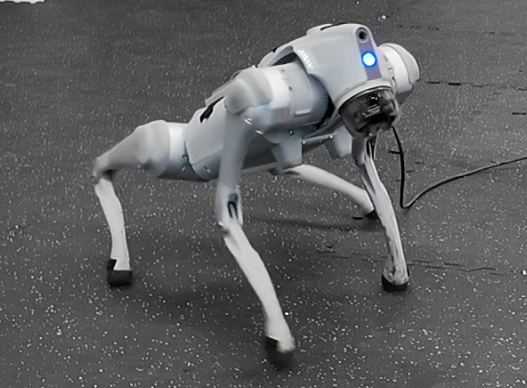
\includegraphics[width=\linewidth]{figure/sim2real_pitch_up.png}
    \end{minipage}
    \begin{minipage}[b]{0.25\linewidth}
        \centering
        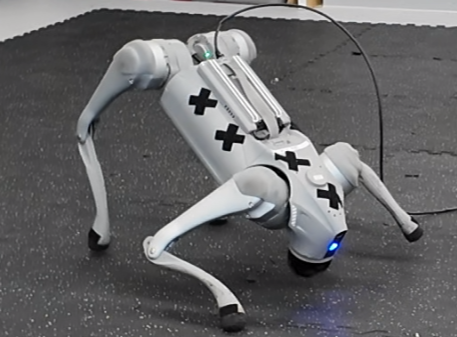
\includegraphics[width=\linewidth]{figure/sim2real_pitch_down.png}
    \end{minipage}
    \begin{minipage}[b]{0.25\linewidth}
        \centering
        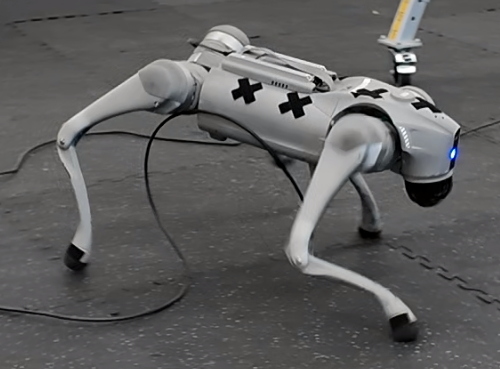
\includegraphics[width=\linewidth]{figure/sim2real_forward.png}
    \end{minipage}
    \caption{\method allows for zero-shot sim2real transfer to Unitree Go2, a commercial quadrupedal robot. }
    \label{fig:sim2real}
\end{figure}